\noindent

Babbie (2015~\cite{babbie2015practice}) states that research is a \textit{"systematic and orderly approach taken towards the collection and analysis of data so that information can be obtained from those data"}
A research methodology establishes the framework for research, amongst other things it defines strategy, approach and components for the research.

Methodologies can be categorised as either qualitative or quantitative and further broken down into approaches such as survey designs, case study, action research, constructivist grounded theory, bibliometric research, design science research, researching history, ethnographic research and experimental research (Williamson \& Johanson (2017~\cite{williamson2017research}).

Over time certain methodologies have been put forward that suite the field of Information Systems which is the chosen field of this work. It is Design Study Research (DSR) which has been selected as the most suitable of these for this particular work. In DSR \textit{"researchers focus on building some kind of artefact they believe will be useful to a particular stakeholder community. They then evaluate the merits of the artefact in various ways"} (Williamson \& Johanson (2017~\cite{williamson2017research}). Figure \ref{fig:typesofresearch} shows the differences between the classic approach, which creates artefacts to attempt to build or test a theory and the DSR approach which builds artefacts that are useful to certain stakeholders.

%https://tex.stackexchange.com/questions/238636/add-caption-to-image-included-with-includegraphics-within-center-environment
\documentclass{article}
\usepackage[demo]{graphicx} % Required for including images
\usepackage[font=small,labelfont=bf]{caption} % Required for specifying captions to tables and figures
\begin{document}
\begin{center}
\begin{minipage}{1\linewidth}
\includegraphics[width=\linewidth]{fig/TypesOfResearch.pdf}
\captionof{figure}{Types of research}
\end{minipage}%
\hfill
\end{center}
\end{document}

Hevner et al. (2004~\cite{hevner2004design}) argued that DSR artefacts can take one of the four forms shown in Figure~\ref{fig:artefactforms}. This definition has not however gained widespread approval and other researchers have put forward differing claims to what defines a DSR approach. Authors such as Gregor and Jones (2007~\cite{gregor2007anatomy}) disagree with this principle and instead suggest a framework where design-research theory is paramount.

\begin{figure}[ht]
    \caption{DSR artefact forms} \label{fig:artefactforms}
    \begin{enumerate}[label=Form \arabic*:, leftmargin=*]
        \item \textbf{Constructs} represent conceptual objects which describe real world "things" such as businesses, employees, levels of debt, sale of products, state of liquidity...

        \item \textbf{Models} represent a subset of real world "things", it is a way by which we can reduce complexity. An example maybe the way we break database systems down into their three sub levels of internal schema, conceptual schema and external schema.

        \item \textbf{Methods} are a set of actions that used together achieve an outcome. The outcome could be a product or a service. One example being test based development which is a method that improves upon software development where the development represents a product.

        \item \textbf{Instantiations} are hardware or software systems that we use produce either a construct, model or method.
    \end{enumerate}
\end{figure}

Indeed one of the issues of DSR is in proving any such research has indeed been done in a rigorous manner as no single approach has been adopted as the gold standard. The approaches that have been put forward include Hevner et al. (2004~\cite{hevner2004design}) which suggests a set of 7 non mandatory guidelines (Table~\ref{tab:HevnerGuidelines}) that should be "addressed in some manner for design-science research to be complete".

% To include draw io image
% https://tex.stackexchange.com/questions/427622/importing-diagram-from-draw-io-into-latex

% Please add the following required packages to your document preamble:
% \usepackage[table,xcdraw]{xcolor}
% If you use beamer only pass "xcolor=table" option, i.e. \documentclass[xcolor=table]{beamer}
%%\begin{table}[]
%%\begin{tabular}{|l|l|l|}
%%\hline
%%\rowcolor[HTML]{C0C0C0} 
%%{\color[HTML]{000000} No.} & {\color[HTML]{000000} Guidelines}            %%               & {\color[HTML]{000000} Explanation}                                                                                                                                                                                                                                                                                                                                                                                                                                                                                                                                                                                                                                                                                                                                                                                                               %%               \\ \hline
%%1                          & Produce a viable artefact                    %%               & \begin{tabular}[c]{@{}l@{}}Design-science research must produce a workable, practical artefact in the form of a construct, model, method, or instantiation.\\ The\end{tabular}                                                                                                                                                                                                                                                                                                                                                                                                                                                                                                                                                                                                                                                                                  \\ \hline
%%2                          & Ensure that the artefact produced is relevant and important & The artefact produced must assist with the resolution of a problem that is deemed relevant and important to some stakeholder community.                                                                                                                                                                                                                                                                                                                                                                                                                                                                                                                                                                                                                                                                                                                         \\ \hline
%%3                          & Rigorously evaluate the artefact produced                   & The effectiveness and efficiency of the artefact must be evaluated using rigorous methods. For instance, it might be evaluated analytically using a mathematical model or empirically using a field study or experiment. The evaluation of an artefact should also include ‘an element of style’, which reflects ‘human perception and taste’.                                                                                                                                                                                                                                                                                                                                                                                                                                                                                                                  \\ \hline
%%4                          & Produce an artefact that makes a research contribution      & \begin{tabular}[c]{@{}l@{}}The artefact produced must make a significant contribution to knowledge via the artefact itself, or the methods used to construct the artefact, or the methods used to evaluate the artefact. For this outcome to occur, the contribution to knowledge must be novel. Moreover, it will be easier to demonstrate a contribution to knowledge if the artefact provides a solution to a previously unsolved problem, or it is uncertain whether a working artefact can even be constructed, or the artefact’s ability to perform ‘appropriately’ is unclear.\\ The\end{tabular}                                                                                                                                                                                                                                                        \\ \hline
%%5                          & Follow rigorous construction methods                        & The artefact must be constructed in a rigorous way. In particular, construction methods must be sufficiently well specified and formalised for other researchers to be able to replicate the way it is constructed. Appropriate levels of rigour should be chosen, however, because excessive rigour can result in the relevance of the artefact being undermined (its usefulness to stakeholders is decreased).                                                                                                                                                                                                                                                                                                                                                                                                                                                \\ \hline
%%6                          & Show the artefact is the outcome of a search process        & \begin{tabular}[c]{@{}l@{}}The artefact should reflect the outcome of a search process whereby available means (actions and resources) are used to reach a desired end under the constraint of ‘laws’ that apply (natural or social laws). The current state of a system (e.g., the artefact being designed) is compared against a goal state. Actions are then taken (sometimes based on heuristics) to reduce the differences between the current and the goal states. The search for actions to reduce differences is iterative until an optimal or a satisfactory solution (match between the current and goal states) is found. To achieve tractable design solutions, the search process often involves simplification and abstraction of the means, ends, and laws and decomposition of the overall problem into simpler sub- problems.\\ 7\end{tabular} \\ \hline
%%7                          & Clearly communicate the research process and outcome        & The research process and outcome must be communicated clearly to stakeholders (both researchers and practitioners). Sufficient detail must be provided to enable (a) the artefact to be constructed and used effectively, and (b) the resources needed to build and use the artefact to be determined.                                                                                                                                                                                                                                                                                                                                                                                                                                                                                                                                                          \\ \hline
%%\end{tabular}
%%\end{table}


\begin{table}[ht]
  \begin{center}
    \caption{Hevner et al. 7 Guidelines for Design-Science Research}
    \label{tab:HevnerGuidelines}
    \begin{tabular}{|l|l|} % <-- Alignments: 1st column left, 2nd middle and 3rd right, with vertical lines in between
      \hline
      \textbf{No.} & \textbf{Guideline}                                          \\
      \hline
      1            & Produce a viable artefact                                   \\
      \hline
      2            & Ensure that the artefact produced is relevant and important \\
      \hline
      3            & Rigorously evaluate the artefact produced                   \\
      \hline
      4            & Produce an artefact that makes a research contribution      \\
      \hline
      5            & Follow rigorous construction methods                        \\
      \hline
      6            & Show the artefact is the outcome of a search process        \\
      \hline
      7            & Clearly communicate the research process and outcome        \\
      \hline
      %      \multirow{2}{*}{Anomaly Detection} & anomaly, anomalous, imbalance, rarity, exception, \\
      %      & oddity, inconsistency, abnormality\\
    \end{tabular}
  \end{center}
\end{table}




%\begin{figure}[htbp]
%\caption{Hevner et al. Guidelines for design-science research} %\label{fig:HevnerGuidelines}
%\begin{table}[]
%\begin{tabular}{|l|l|}
%\hline
%{No.} & {Guidelines}           \\ \hline
%1                          & Produce a viable artefact                     %              \\ \hline
%2                          & Ensure that the artefact produced is relevant %and important \\ \hline
%3                          & Rigorously evaluate the artefact produced     %              \\ \hline
%4                          & Produce an artefact that makes a research %contribution      \\ \hline
%5                          & Follow rigorous construction methods          %              \\ \hline
%6                          & Show the artefact is the outcome of a search %process        \\ \hline
%7                          & Clearly communicate the research process and %outcome        \\ \hline
%\end{tabular}
%\end{table}
%\end{figure}



%\begin{figure}[htbp]
%\caption{Hevner et al. Guidelines for design-science research} %\label{fig:HevnerGuidelines}

%\begin{enumerate}[leftmargin=*]
%    \item Produce a viable artefact%. Design-science research must produce a workable, practical artefact in the form of a construct, model, method, or instantiation.

%    \item Ensure that the artefact produced is relevant and important%. The artefact produced must assist with the resolution of a problem that is deemed relevant and important to some stakeholder community.

%    \item Rigorously evaluate the artefact produced%. The effectiveness and efficiency of the artefact must be evaluated using rigorous methods. For instance, it might be evaluated analytically using a mathematical model or empirically using a field study or experiment. The evaluation of an artefact should also include ‘an element of style’, which reflects ‘human perception and taste’.

%    \item Produce an artefact that makes a research contribution%. The artefact produced must make a significant contribution to knowledge via the artefact itself, or the methods used to construct the artefact, or the methods used to evaluate the artefact. For this outcome to occur, the contribution to knowledge must be novel. Moreover, it will be easier to demonstrate a contribution to knowledge if the artefact provides a solution to a previously unsolved problem, or it is uncertain whether a working artefact can even be constructed, or the artefact’s ability to perform ‘appropriately’ is unclear.

%    \item Follow rigorous construction methods%. The artefact must be constructed in a rigorous way. In particular, construction methods must be sufficiently well specified and formalised for other researchers to be able to replicate the way it is constructed. Appropriate levels of rigour should be chosen, however, because excessive rigour can result in the relevance of the artefact being undermined (its usefulness to stakeholders is decreased).

%    \item Show the artefact is the outcome of a search process%. The artefact should reflect the outcome of a search process whereby available means (actions and resources) are used to reach a desired end under the constraint of ‘laws’ that apply (natural or social laws). The current state of a system (e.g., the artefact being designed) is compared against a goal state. Actions are then taken (sometimes based on heuristics) to reduce the differences between the current and the goal states. The search for actions to reduce differences is iterative until an optimal or a satisfactory solution (match between the current and goal states) is found. To achieve tractable design solutions, the search process often involves simplification and abstraction of the means, ends, and laws and decomposition of the overall problem into simpler sub- problems.

%    \item Clearly communicate the research process and outcome%. The research process and outcome must be communicated clearly to stakeholders (both researchers and practitioners). Sufficient detail must be provided to enable (a) the artefact to be constructed and used effectively, and (b) the resources needed to build and use the artefact to be determined.
%\end{enumerate}

%\end{figure}


A number of concerns of this approach have been pointed out by academics, including its generic applicability to other types of research apart from DSR and the difficulty in gauging some of the guideline's aims. For instance what makes an artefact viable or how do we know when an artefact has been produced rigorously?

Gregor and Jones (2007~\cite{gregor2007anatomy}) does not suffer from this generic criticism. They put forward an approach which looks at design-science theory and states that design-science theory has 6 obligatory components and potentially a further 2 optional ones (Table~\ref{tab:GregorGuidelines}).

\begin{table}[ht]
  \begin{center}
    \caption{Gregor and Jones's 8 Guidelines for Design-Science Theory}
    \label{tab:GregorGuidelines}
    \begin{tabular}{|l|l|} % <-- Alignments: 1st column left, 2nd middle and 3rd right, with vertical lines in between
      \hline
      \textbf{No.} & \textbf{Guideline}                            \\
      \hline
      1            & Purpose and scope                             \\
      \hline
      2            & Constructs                                    \\
      \hline
      3            & Form and function                             \\
      \hline
      4            & Mutability                                    \\
      \hline
      5            & Testable propositions                         \\
      \hline
      6            & Justifactory knowledge                        \\
      \hline
      7            & Implementation principles \textit{(Optional)} \\
      \hline
      8            & Instantiation \textit{(Optional)}             \\
      \hline
      %      \multirow{2}{*}{Anomaly Detection} & anomaly, anomalous, imbalance, rarity, exception, \\
      %      & oddity, inconsistency, abnormality\\
    \end{tabular}
  \end{center}
\end{table}

Again this approach has suffered criticism in giving only minimum guidance in the pursuit of research rigour. Another criticism is it only considers 'method' and 'product' artefacts from the 4 possibilities mentioned in Figure~\ref{fig:artefactforms} that defines DSR.

Peffers et al. (2007~\cite{peffers2007design}) suggest a research methodology using a six step process for correct implementation of DSR (Table~\ref{tab:PefferGuidelines}). Through these steps Peffers et al. claim they are able to confirm design-science research which is "valuable, rigorous, publishable". Others have made similar claims with many frameworks having some comparable ideas along with their own strengths and weaknesses. Many practitioners advise that you simply choose one that fits your research and then simply adhere to it rigorously.

Objectives that a researcher must conform to demonstrate well structured DSR should show clearly that they understand the problem at hand and not jump to a solution first approach. Do not create a 'solution looking for a problem'. In describing the problem they must specify who is experiencing the problem, what is the nature of the problem and success criteria. Why this problem can't be solved with existing means. When the problem arises, where it occurs and stakeholders affected by it. Through covering all these questions the researcher is explaining they understand the nature and boundary of the problem. The boundary of a problem is important as too narrow a scope would be considered uninteresting in the research community and too wide a scope, impractical.

\begin{table}[ht]
  \begin{center}
    \caption{Peffers et al. 6 Step Iterative Process for Conducting DSR}
    \label{tab:PefferGuidelines}
    \begin{tabular}{|l|l|} % <-- Alignments: 1st column left, 2nd middle and 3rd right, with vertical lines in between
      \hline
      \textbf{No.}       & \textbf{Step}                                                        \\
      \hline
      1                  & Identify, define, and motivate the focal problem                     \\
      \hline
      \multirow{2}{*}{2} & Define objectives that a solution (possibly partial)                 \\
                         & to the focal problem must achieve                                    \\
      \hline
      3                  & Design and develop the artefact                                      \\
      \hline
      4                  & Demonstrate the artefact can be used to help solve the focal problem \\
      \hline
      5                  & Evaluate how well the artefact solves the focal problem              \\
      \hline
      6                  & Communicate the outcomes of the research                             \\
      \hline
    \end{tabular}
  \end{center}
\end{table}


% https://tex.stackexchange.com/questions/64836/change-image-size#64843
%\includegraphics[width=0.9\columnwidth]{TypesOfResearch.pdf}
%\begin{figure}[!htb]
%  \includegraphics[width=0.9\columnwidth]{fig/TypesOfResearch.pdf}
%  \caption{Types of research within information systems}
%  \label{fig:typesofresearch}
%\end{figure}

%% Please add the following required packages to your document preamble:
% \usepackage[table,xcdraw]{xcolor}
% If you use beamer only pass "xcolor=table" option, i.e. \documentclass[xcolor=table]{beamer}
%%\begin{table}[]
%%\begin{tabular}{|l|l|l|}
%%\hline
%%\rowcolor[HTML]{C0C0C0} 
%%{\color[HTML]{000000} No.} & {\color[HTML]{000000} Guidelines}            %%               & {\color[HTML]{000000} Explanation}                                                                                                                                                                                                                                                                                                                                                                                                                                                                                                                                                                                                                                                                                                                                                                                                               %%               \\ \hline
%%1                          & Produce a viable artefact                    %%               & \begin{tabular}[c]{@{}l@{}}Design-science research must produce a workable, practical artefact in the form of a construct, model, method, or instantiation.\\ The\end{tabular}                                                                                                                                                                                                                                                                                                                                                                                                                                                                                                                                                                                                                                                                                  \\ \hline
%%2                          & Ensure that the artefact produced is relevant and important & The artefact produced must assist with the resolution of a problem that is deemed relevant and important to some stakeholder community.                                                                                                                                                                                                                                                                                                                                                                                                                                                                                                                                                                                                                                                                                                                         \\ \hline
%%3                          & Rigorously evaluate the artefact produced                   & The effectiveness and efficiency of the artefact must be evaluated using rigorous methods. For instance, it might be evaluated analytically using a mathematical model or empirically using a field study or experiment. The evaluation of an artefact should also include ‘an element of style’, which reflects ‘human perception and taste’.                                                                                                                                                                                                                                                                                                                                                                                                                                                                                                                  \\ \hline
%%4                          & Produce an artefact that makes a research contribution      & \begin{tabular}[c]{@{}l@{}}The artefact produced must make a significant contribution to knowledge via the artefact itself, or the methods used to construct the artefact, or the methods used to evaluate the artefact. For this outcome to occur, the contribution to knowledge must be novel. Moreover, it will be easier to demonstrate a contribution to knowledge if the artefact provides a solution to a previously unsolved problem, or it is uncertain whether a working artefact can even be constructed, or the artefact’s ability to perform ‘appropriately’ is unclear.\\ The\end{tabular}                                                                                                                                                                                                                                                        \\ \hline
%%5                          & Follow rigorous construction methods                        & The artefact must be constructed in a rigorous way. In particular, construction methods must be sufficiently well specified and formalised for other researchers to be able to replicate the way it is constructed. Appropriate levels of rigour should be chosen, however, because excessive rigour can result in the relevance of the artefact being undermined (its usefulness to stakeholders is decreased).                                                                                                                                                                                                                                                                                                                                                                                                                                                \\ \hline
%%6                          & Show the artefact is the outcome of a search process        & \begin{tabular}[c]{@{}l@{}}The artefact should reflect the outcome of a search process whereby available means (actions and resources) are used to reach a desired end under the constraint of ‘laws’ that apply (natural or social laws). The current state of a system (e.g., the artefact being designed) is compared against a goal state. Actions are then taken (sometimes based on heuristics) to reduce the differences between the current and the goal states. The search for actions to reduce differences is iterative until an optimal or a satisfactory solution (match between the current and goal states) is found. To achieve tractable design solutions, the search process often involves simplification and abstraction of the means, ends, and laws and decomposition of the overall problem into simpler sub- problems.\\ 7\end{tabular} \\ \hline
%%7                          & Clearly communicate the research process and outcome        & The research process and outcome must be communicated clearly to stakeholders (both researchers and practitioners). Sufficient detail must be provided to enable (a) the artefact to be constructed and used effectively, and (b) the resources needed to build and use the artefact to be determined.                                                                                                                                                                                                                                                                                                                                                                                                                                                                                                                                                          \\ \hline
%%\end{tabular}
%%\end{table}


\begin{table}[ht]
  \begin{center}
    \caption{Hevner et al. 7 Guidelines for Design-Science Research}
    \label{tab:HevnerGuidelines}
    \begin{tabular}{|l|l|} % <-- Alignments: 1st column left, 2nd middle and 3rd right, with vertical lines in between
      \hline
      \textbf{No.} & \textbf{Guideline}                                          \\
      \hline
      1            & Produce a viable artefact                                   \\
      \hline
      2            & Ensure that the artefact produced is relevant and important \\
      \hline
      3            & Rigorously evaluate the artefact produced                   \\
      \hline
      4            & Produce an artefact that makes a research contribution      \\
      \hline
      5            & Follow rigorous construction methods                        \\
      \hline
      6            & Show the artefact is the outcome of a search process        \\
      \hline
      7            & Clearly communicate the research process and outcome        \\
      \hline
      %      \multirow{2}{*}{Anomaly Detection} & anomaly, anomalous, imbalance, rarity, exception, \\
      %      & oddity, inconsistency, abnormality\\
    \end{tabular}
  \end{center}
\end{table}




%\begin{figure}[htbp]
%\caption{Hevner et al. Guidelines for design-science research} %\label{fig:HevnerGuidelines}
%\begin{table}[]
%\begin{tabular}{|l|l|}
%\hline
%{No.} & {Guidelines}           \\ \hline
%1                          & Produce a viable artefact                     %              \\ \hline
%2                          & Ensure that the artefact produced is relevant %and important \\ \hline
%3                          & Rigorously evaluate the artefact produced     %              \\ \hline
%4                          & Produce an artefact that makes a research %contribution      \\ \hline
%5                          & Follow rigorous construction methods          %              \\ \hline
%6                          & Show the artefact is the outcome of a search %process        \\ \hline
%7                          & Clearly communicate the research process and %outcome        \\ \hline
%\end{tabular}
%\end{table}
%\end{figure}



%\begin{figure}[htbp]
%\caption{Hevner et al. Guidelines for design-science research} %\label{fig:HevnerGuidelines}

%\begin{enumerate}[leftmargin=*]
%    \item Produce a viable artefact%. Design-science research must produce a workable, practical artefact in the form of a construct, model, method, or instantiation.

%    \item Ensure that the artefact produced is relevant and important%. The artefact produced must assist with the resolution of a problem that is deemed relevant and important to some stakeholder community.

%    \item Rigorously evaluate the artefact produced%. The effectiveness and efficiency of the artefact must be evaluated using rigorous methods. For instance, it might be evaluated analytically using a mathematical model or empirically using a field study or experiment. The evaluation of an artefact should also include ‘an element of style’, which reflects ‘human perception and taste’.

%    \item Produce an artefact that makes a research contribution%. The artefact produced must make a significant contribution to knowledge via the artefact itself, or the methods used to construct the artefact, or the methods used to evaluate the artefact. For this outcome to occur, the contribution to knowledge must be novel. Moreover, it will be easier to demonstrate a contribution to knowledge if the artefact provides a solution to a previously unsolved problem, or it is uncertain whether a working artefact can even be constructed, or the artefact’s ability to perform ‘appropriately’ is unclear.

%    \item Follow rigorous construction methods%. The artefact must be constructed in a rigorous way. In particular, construction methods must be sufficiently well specified and formalised for other researchers to be able to replicate the way it is constructed. Appropriate levels of rigour should be chosen, however, because excessive rigour can result in the relevance of the artefact being undermined (its usefulness to stakeholders is decreased).

%    \item Show the artefact is the outcome of a search process%. The artefact should reflect the outcome of a search process whereby available means (actions and resources) are used to reach a desired end under the constraint of ‘laws’ that apply (natural or social laws). The current state of a system (e.g., the artefact being designed) is compared against a goal state. Actions are then taken (sometimes based on heuristics) to reduce the differences between the current and the goal states. The search for actions to reduce differences is iterative until an optimal or a satisfactory solution (match between the current and goal states) is found. To achieve tractable design solutions, the search process often involves simplification and abstraction of the means, ends, and laws and decomposition of the overall problem into simpler sub- problems.

%    \item Clearly communicate the research process and outcome%. The research process and outcome must be communicated clearly to stakeholders (both researchers and practitioners). Sufficient detail must be provided to enable (a) the artefact to be constructed and used effectively, and (b) the resources needed to build and use the artefact to be determined.
%\end{enumerate}

%\end{figure}

